\chapter{Block preconditioning of the Stokes equations}
\noindent
\modinfo{Module name}{Stokes}
\modinfo{Module subroutines}{StokesSolver}
\modinfo{Module authors}{Mika Malinen}
\modinfo{Document authors}{Mika Malinen}
\modinfo{Document edited}{Feb 20th 2006}

\section{Introduction}

The discretization of flow equations leads usually to large linear systems. Since
the direct solution of large linear systems is often too expensive in computation time 
and computer memory requirements, such linear systems are customarily solved
with iterative algorithms, in combination with preconditioning.
%For a discussion of key ideas underlying the preconditioned solution methods
%see, for example, \cite{ESW05}.

The general preconditioning strategy used in Elmer is based on the computation of 
incomplete factorizations. The performance of these preconditioners 
is case-dependent and may
not always be satisfactory. More efficient solution algorithms for a particular
problem can often be developed by exploiting the block structure of the 
linear system. This strategy has been used to develop an alternative
solution method for the linear systems which result from the discretization
of the Stokes equations. In the following a description of this solution 
method will be given.

It should be noted that in Elmer the Stokes equations can be solved with the solver 
for the Navier-Stokes equations. The alternative
solution method described here can however be applied only in connection with 
a special solver for the Stokes equations. This special solver is still
under development and a lot of additional features accessible through 
the Navier-Stokes solver are not available currently.       
Suggestions concerning the further development of this special solver are welcome.   


\section{Theory}

The solver described here can be used to solve numerically the  
Stokes equations.
%accompanied by suitable mixed boundary conditions.
In the evolutionary case the field equations are given by
\begin{equation}\label{stokes_system}
\begin{split}
\rho\frac{\partial\vec u}{\partial t} - \mu \Delta\vec u +\nabla p &= \vec b, \\
\nabla \cdot \vec u &= 0.
\end{split}
\end{equation}
The velocity boundary conditions of Dirichlet type or
homogeneous natural boundary conditions can be imposed on the boundary.
It is noted that
the uniqueness of the pressure solution is assumed to be 
ensured by imposing the normal natural boundary condition        
\begin{equation}\label{Neumann-outflow}
-p + \mu (\nabla\vec u)\vec n\cdot\vec n = 0
%\frac{\partial\vec u}{\partial n} = 0
\end{equation}
on a nontrivial part of the boundary. 

When a boundary can be represented as a coordinate plane,
slip boundary conditions may also given. In the case of slip
boundary condition it is assumed that the normal velocity is prescribed
to vanish ($u_n = \vec u \cdot \vec n = 0$) and the tangential
surface force $s_s$ is related to the tangential velocity $u_s$ by
\begin{equation}\label{slipbc}
s_s = \mu \frac{\partial u_s}{\partial n} = -C_n u_s.
\end{equation}
Here the subscript $s$ refers to the tangential direction and 
$C_n$ is the slip coefficient for the boundary (the subscript $n$ refers to
the normal direction).

If the alternative solution strategy is applied,  
the finite element discretization of (\ref{stokes_system}) is assumed to be 
based on the lowest equal order approximation for the velocity and pressure. 
Such discretization of (\ref{stokes_system}) leads to a linear system 
\begin{equation}\label{discrete-stokes-system}
Ky=b
\end{equation}
where $K$ has the block-structure
\begin{equation}\label{block-structure}
K=\left( \begin{array}{cc} A    & B^T \\
                         B    & C   \end{array}\right). 
\end{equation}
Here $A$ is the coefficient matrix which results from the discretization 
of $-\mu\Delta \vec u$ or the spatial and backward Euler time discretization of
$\rho(\partial\vec u /\partial t) -\mu\Delta \vec u$.
In addition, $C$ is a stabilization matrix
which results from adding a stabilization operator suggested in \cite{Do04}.
%in the case of the lowest equal order approximation.

The iterative solution methods considered here are based on applying a
Krylov subspace method to (\ref{discrete-stokes-system}) 
in combination with a block-preconditioner
\begin{equation}
P= \left( \begin{array}{cc} P_A           & B^T \\
                         0    & P_S   \end{array}\right)  
\end{equation}
where $P_A$ and $P_S$ 
approximate $A$ and the Schur complement of $A$ in $K$.  
In practice, the application of the preconditioner requires that the actions of the inverses 
$P_A^{-1}$ and $P_S^{-1}$ are approximated. 
These tasks can often be done efficiently by applying iterative methods to systems
of type $P_Az_A=r_A$ and $P_Sz_S=r_S$.

The action of the inverse of $P_S$ is constructed in such a way that one has 
in the stationary case \cite{Si94} 
\begin{equation}\label{stationaryPs}
P_S^{-1}r_S \approx -(\frac{1}{\mu}M)^{-1}r_S   
\end{equation}
and in the evolutionary case \cite{Ca88}
\begin{equation}\label{evolutionaryPs}
P_S^{-1}r_S \approx (\frac{\delta t}{\rho}D)^{-1}r_S - (\frac{1}{\mu}M)^{-1}r_S    
\end{equation}
where $r_S$ is a vector in the pressure space, $\delta t$ is the size of time step, and 
$M$ and $D$ are finite element approximations of the identity 
and Laplace operators. It is noted that the Laplace operator in (\ref{evolutionaryPs})
is associated with the homogeneous Dirichlet boundary condition on the part of the boundary
where the boundary condition (\ref{Neumann-outflow}) is given,
while the homogeneous Neumann boundary condition is used on the remaining part
of the boundary.

It is noted that 
the actions of the approximate inverses of the scaled pressure mass matrices in 
(\ref{stationaryPs}) and (\ref{evolutionaryPs}) are always computed 
with the BICGSTAB method. The user can choose a method for 
approximating the action of the inverse of the pressure Laplacian operator in (\ref{evolutionaryPs}).
Several options such as applying an algebraic multigrid V-cycle are available for this computation. 

In the stationary case each action of the preconditioner
depends upon an approximate solution of a Poisson equation for each of the velocity components.
The user can choose a method for this computation.  
In the evolutionary case the action of the inverse of $P_A$ 
is always computed with the BICGSTAB method. 

The outer iterative method which is applied to (\ref{discrete-stokes-system})
is based on either BICGSTAB method or a nested GCR algorithm.
The nested GCR algorithm is based on the idea of solving the new search direction
of the outer GCR iteration from the residual equation which characterizes the 
error in the current approximate solution. The residual equation is solved 
approximately by taking at most $m$ steps of the block-preconditioned GCR algorithm
where $m$ can be controlled by the user.

It is mentioned that 
the method based on BICGSTAB has the benefit of requiring only a small, fixed amount 
of computer memory. A drawback is that the performance may deteriorate when
more inaccurate solutions of preconditioning systems are allowed. 
The nested GCR algorithm has been found to perform robustly with respect to 
inaccuracies in preconditioning, but as compared with BICGSTAB more solution
vectors may need to be saved during the iteration.  


 
  
  
 


\section{Keywords}

\sifbegin
\sifitemnt{Material}{material-id}
\sifbegin
\sifitem{Density}{Real} 
This keyword is used to define the density $\rho$.

\sifitem{Viscosity}{Real} 
This keyword is used to define the viscosity $\mu$.

\sifend
\sifend


\sifbegin
\sifitemnt{Solver}{solver-id}
\sifbegin

\sifitem{Equation}{String}
This keyword declares the name of the equation.

\sifitem{Procedure}{File ''Stokes'' ''StokesSolver''}
The name of the file and procedure.

\sifitem{Variable}{String ''Stokes''}
This keyword declares the name of the solution.

\sifitem{Variable Dofs}{Integer}
The value of this keyword defines the number of unknown scalar fields
and must hence equal to $d+1$ where $d$ is the spatial 
dimensionality of the computational domain.
It is noted that the unknown scalar fields are always numbered in such a
way that the highest running number is associated with the pressure
solution. 

\sifitem{Stabilize}{Logical}
By default this keyword is given the value {\tt ''True''} so that
the equal order approximation for the velocity and pressure may be used.

\sifitem{Block Preconditioning}{Logical} 
If the block preconditioning is used, the value of this keyword must 
be {\tt ''True''}. 

\sifitem{Outer Iteration Method}{String}
This keyword is used to define the outer iterative method.
The default method is the nested GCR algorithm. 
In order to use the method based on BICGSTAB the value {\tt ''BICGSTAB''} should be given
for this keyword.  

\sifitem{Max Outer Iterations}{Integer}
When the outer iterative method is based on BICGSTAB,
the value of this keyword defines the maximum number of outer iterations allowed,
i.e. the maximum number of the block preconditioned  
iterations. When the outer iterative method is 
the nested GCR algorithm, this keyword is used to
control restarting so that the outer GCR algorithm is restarted
after each $m$ iteration steps where $m$ is the value of this keyword.

\sifitem{Max Outer GCR Cycles}{Integer}
When the outer iterative method is
the nested GCR algorithm, the value of this keyword defines the maximum number
of restarts allowed in the outer GCR iteration. 
The default value is the unity which corresponds to allowing only one
GCR cycle.

\sifitem{Use Truncation}{Logical}
When the outer iterative method is the nested GCR algorithm,
a truncation strategy may be used in combination with restarting.
If the value {\tt ''True''} is given for this keyword, after restarting
the orthogonalization of the new search direction vector is done
with respect to $m$ previously used search direction vectors where
$m$ is the value of {\tt Max Outer Iterations}
keyword.

\sifitem{Max Inner GCR Iterations}{Integer}
When the outer iterative method is the nested GCR algorithm, 
the value of this keyword defines the maximum number
of inner GCR iterations (it is noted that restarting cannot be used 
in connection with inner GCR iterations)

\sifitem{Linear System Convergence Tolerance}{Real}
When the block preconditioning is used, the value of this keyword defines
the convergence tolerance used in connection with the solution of preconditioning systems.
Ideally, one should try to use a rather large value so that
the cost of preconditioning is not excessive.  

\sifitem{Linear System Max Iterations}{Integer}
When the block preconditioning is used, this keyword is used to define
the maximum number of iterations allowed in the solution of
preconditioning systems of type $P_Az_A=r_A$ and $P_Sz_S=r_S$.

\sifitem{Ratio of Convergence Tolerances}{Real}
This keyword is used to define the convergence tolerance $TOL$ for 
outer iterations. The value of this keyword defines the ratio of   
TOL to the convergence tolerance used in connection with the solution of 
preconditioning systems. Here the convergence tolerance for 
the solution of preconditioning systems is defined
using the {\tt Linear System Convergence Tolerance} keyword. 

\sifitem{Residual Reduction Ratio}{Real}
When the outer iterative method is the nested GCR algorithm,
this keyword may be used to define a stopping criterion 
for the inner GCR iterations (cf.\ the use of 
{\tt Max Inner GCR Iterations} keyword).
The inner GCR iteration is stopped when the new search vector so obtained
is guaranteed to
reduce the norm of the outer iteration residual by a ratio $\epsilon$ where
$\epsilon$ is the value of this keyword.
The default value of this keyword is 0.1.


\sifitem{ILU Order for Schur Complement}{Integer}
In the stationary case the value of this keyword defines 
the fill level for the incomplete LU factorization preconditioner that 
is used in the iterative solution of the linear systems   
involving $P_S$. In the evolutionary case this keyword may be used to
define an incomplete factorization preconditioner for the pressure mass 
matrix $M$ in (\ref{evolutionaryPs}). It should be noted that
in the evolutionary case the usual linear
solver keywords can be used to define an iterative method for the solution of
the pressure Laplacian system in (\ref{evolutionaryPs}). 
It is also noted that if 
the value of this keyword is not given, then
the Jacobi preconditioning will be used instead of incomplete 
factorization preconditioning.

\sifitem{ILU Order for Velocities}{Integer}
In the evolutionary case this keyword may be used to
define an incomplete factorization preconditioner which is 
used in conjuction with the approximation of the action of $P_A^{-1}$.
If the value of this keyword is not given, then
the Jacobi preconditioning will be used instead of incomplete 
factorization preconditioning.
It should be noted that
in the stationary case the usual linear
solver keywords can be used to define an iterative method for the solution of
the systems involving $P_A$.



\sifend
\sifend


\sifbegin
\sifitemnt{Body Force}{bf-id}
\sifbegin

\sifitem{Body Force i}{Real}
This keyword is used to define the i's component of the body force vector $\vec b$.

\sifend
\sifend




\sifbegin
\sifitemnt{Boundary Condition}{bc-id}
\sifbegin

\sifitem{Outflow boundary}{Logical}
If the value {\tt ''True''} is given
for this keyword, then the outflow boundary condition (\ref{Neumann-outflow}) 
will be used.

\sifitem{Slip Boundary}{Logical}
If the slip boundary condition is defined, then the value {\tt ''True''}
must be given for this keyword.

\sifitem{Slip Coefficient i}{Real}
The value of the slip coefficient in (\ref{slipbc}).
Here $i$ refers to the coordinate direction which is parallel to the normal 
direction of the boundary.




\sifend
\sifend

\begin{figure}[h]
  \vspace{-3cm}
  \begin{center}
    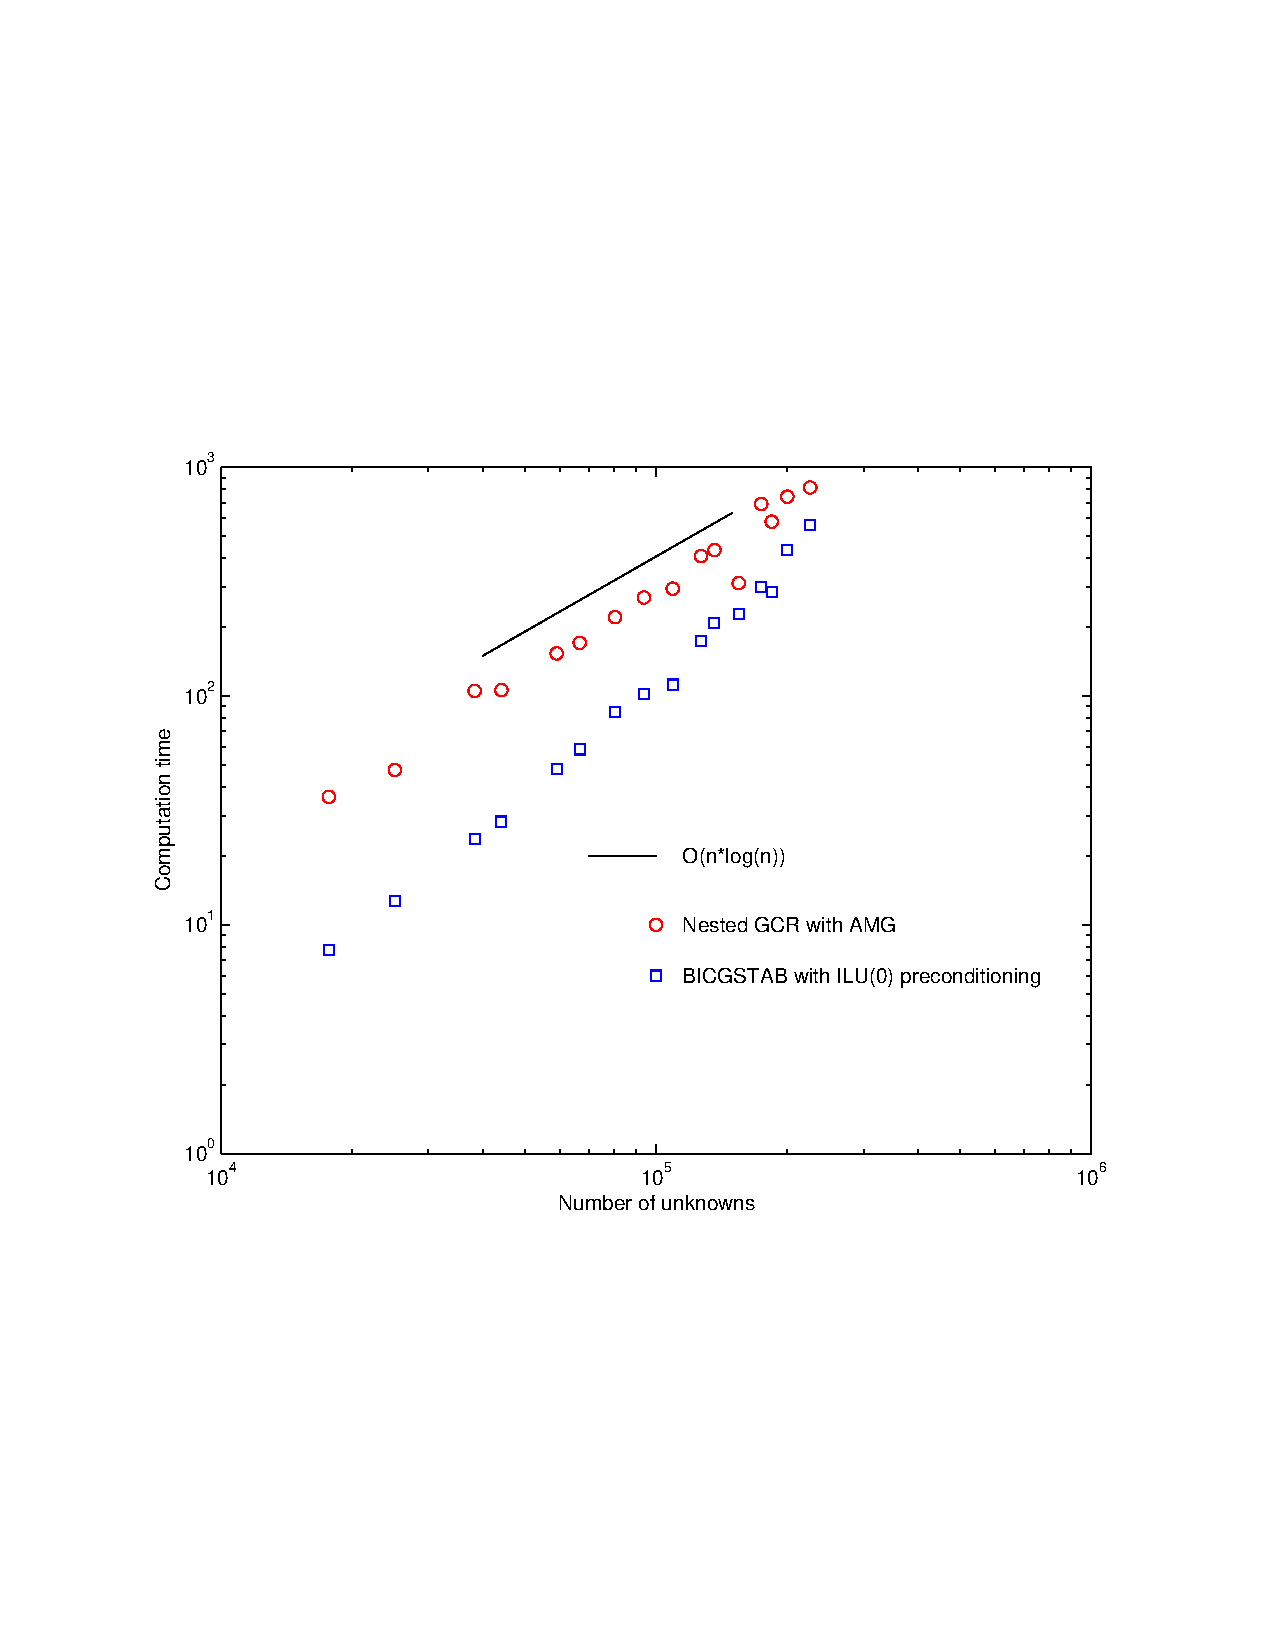
\includegraphics[width=0.49\textwidth]{comptime.pdf}
    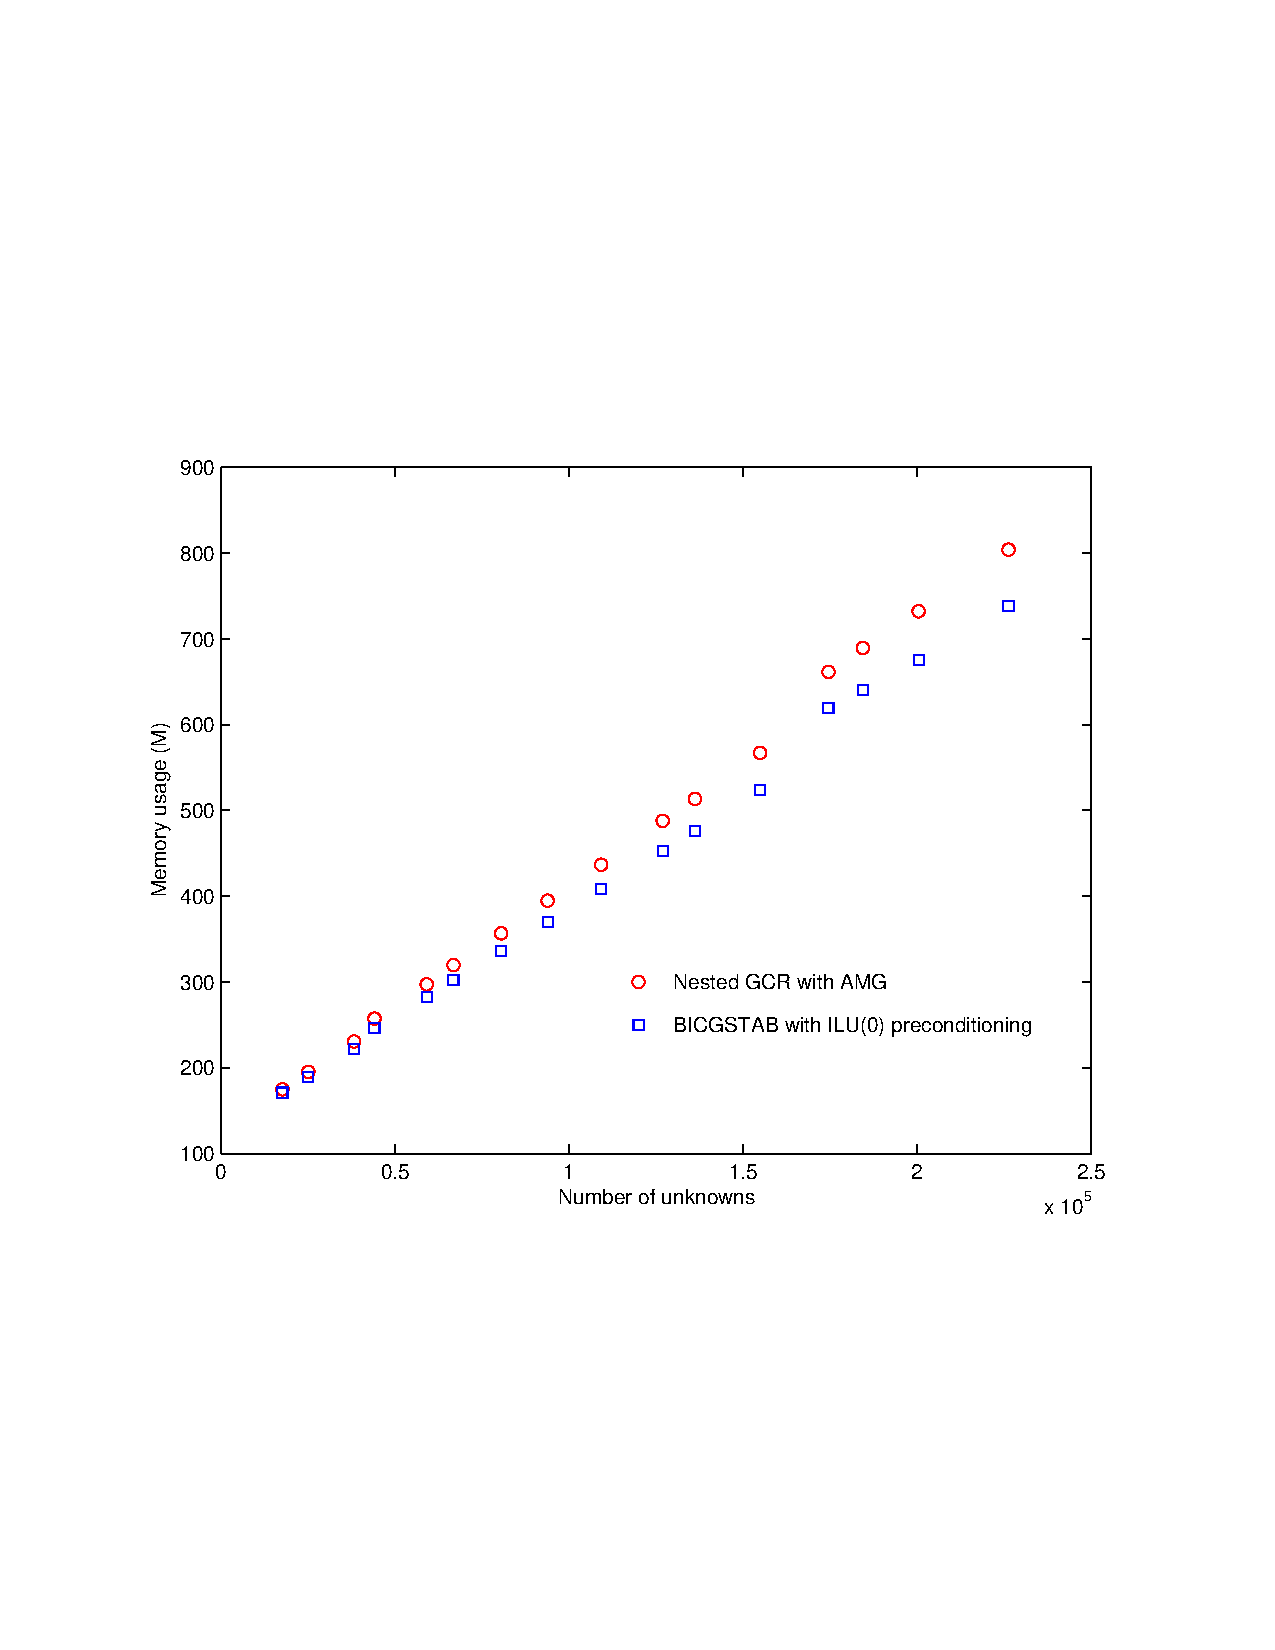
\includegraphics[width=0.49\textwidth]{memory.pdf}
   \end{center}
  \vspace{-3cm}
\caption{A comparison of the nested GCR algorithm with the ILU(0) preconditioned
BICGSTAB method in the case of a three-dimensional test problem. 
In the nested GCR algorithm the algebraic multigrid (AMG) solver was used to 
compute the action of $P_A^{-1}$.}
\end{figure}


\bibliography{elmerbib}
\bibliographystyle{plain}

